
Function inlining, or simply inlining, is a classic code
transformation that can significantly increase the performance of many
programs.  A compiler pass that decides which calls to inline, and in
which order, is referred to as an inliner.  The basic idea of inlining
is straightforward: rather than making a function call, replace the
call in the originating function with a copy of the body of the
to-be-called function.  Nonetheless, many inliner designs are
possible; \cite{BerubePhD} describes the existing inliner
in \llvm, and also the alternative
approach used by a new feedback-directed inliner (\FDI) that uses \CP.
All inlining discussed in this paper is implemented in the
open-source \llvm\ compiler~\cite{LattnerAdveCGO04}.

Some terminology is required to identify the various functions and
calls involved in the inlining process.  The function making a call is
referred to as the {\it caller}, while the called function is the {\it
callee}.  The representation of a call in a compiler's {\it internal
representation} (IR) is a {\it call site}; in \llvm, a call site is an
instruction that indicates both the caller and the callee.  Thus,
inlining replaces a call site by a copy of that call site's callee.
When a call is inlined, the callee may contain call sites, which are
copied into the caller to produce new call sites.  The call site where
inlining occurs is called the {\it source} call site.  A call site in
the callee that is copied during inlining is called an {\it original}
call site, and the new copy of the original call site inside the
caller is called the {\it target} call site.

\subsection{Barriers to Inlining}

Not every call site can be inlined.  Indirect calls use a pointer
variable to identify the location of the called code, and arise from
function pointers and dynamically-polymorphic call dispatching.  These
calls cannot be inlined, because the callee is unknown at compiler
time.  External calls into code not currently available in the
compiler, such as calls into different modules or to statically-linked
library functions cannot be inlined before link-time because the
source representation of the callee is not available in the compiler.
Calls to dynamically-linked libraries can never be inlined by
definition. Moreover, if a callee uses a \name{setjump} instruction,
it cannot be inlined. A \name{setjump} can redirect program control
flow {\it anywhere}, including the middle of different function,
without using the call/return mechanisms.  Inlining the \name{setjump}
could cause any manual stack management at the target of the jump to be
incorrect; the inlined version would not be functionally equivalent to
the original.

\subsection{Benefits of Inlining}

Inlining a call has a small direct benefit.  Removing the call reduces
the number of executed instructions.  The {\tt call} instruction in
the caller is unnecessary, as is the {\tt return} instruction in the
callee.  Furthermore, any parameters passed to the callee and any
values returned no longer need to be pushed onto the
stack\footnote{Some calling conventions allow values to pass between
  the caller and callee in registers.}.

\begin{figure}
  \centering
  
  \begin{minipage}[t]{\linewidth}
    \subfigure[Original code fragment] {
      \begin{minipage}[b]{0.45\textwidth}
        \centering
        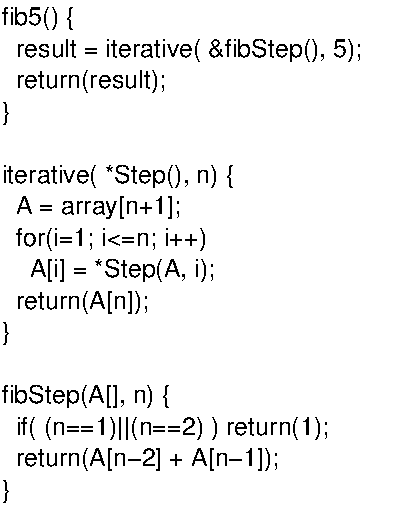
\includegraphics[height=12em]{Figures/fibiter-1}
      \end{minipage}
      \label{fibiter:orig}
    }
    \subfigure[after inlining \iname{iterative}] {
      \begin{minipage}[b]{0.45\textwidth}
        \centering
        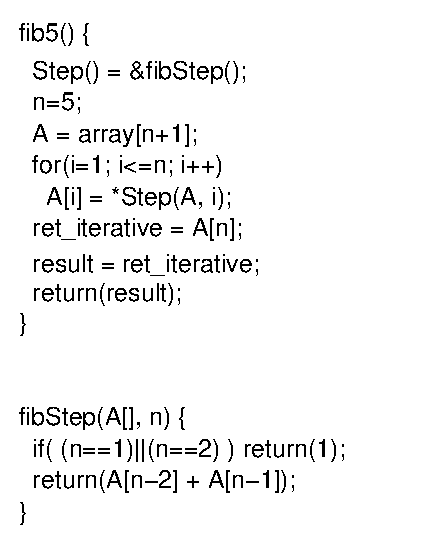
\includegraphics[height=12em]{Figures/fibiter-2}
      \end{minipage}
      \label{fibiter:iterative}
    }
    \vspace{1em}
    \hrule
    \vspace{1em}
  \end{minipage}
  \begin{minipage}[t]{\linewidth}
    \centering
    \subfigure[after constant and copy propagation] {
      \begin{minipage}[b]{0.40\linewidth}
        \centering
        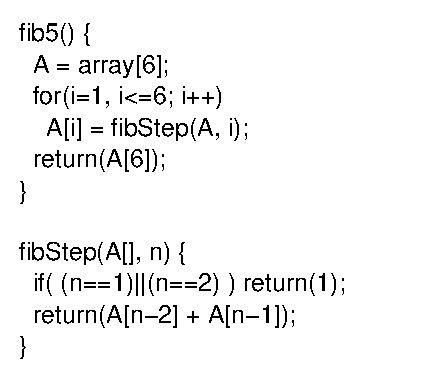
\includegraphics[height=8.8em]{Figures/fibiter-3}
      \end{minipage}
      \label{fibiter:prop}
    }
    \hspace{0.07\linewidth}
    \subfigure[after inlining \iname{fibStep} and simplification] {
      \begin{minipage}[b]{0.40\linewidth}
        \centering
        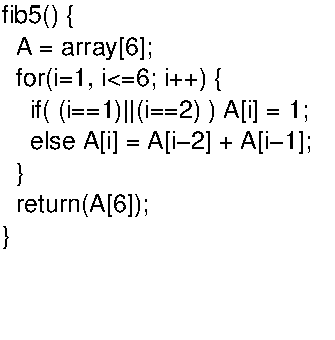
\includegraphics[height=8.8em]{Figures/fibiter-4}
      \end{minipage}
      \label{fibiter:fibstep}
    }
    \vspace{1em}
    \hrule
    \vspace{1em}
    \hspace{0.07\linewidth}
    \subfigure[after loop unrolling and scalar promotion] {
      \begin{minipage}[b]{0.34\linewidth}
        \centering
        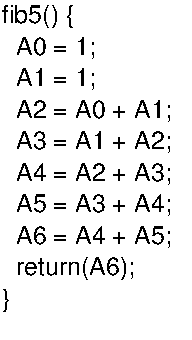
\includegraphics[height=8.8em]{Figures/fibiter-5}
      \end{minipage}
      \label{fibiter:final}
    }
  \end{minipage}
  \caption{A sequence of transformations on a code fragment that
    computes Fibonacci numbers, illustrating the code-simplification
    opportunities enabled by inlining ~\cite{BerubePhD}}
  \label{fig:fibiter}
\end{figure}

However, the greatest potential benefit of inlining comes from
additional code simplification it may enable by bringing the callee's
code into the caller's scope. \refFigure{fig:fibiter} presents a
running example demonstrating the transformations that become possible
due to inlining.  Many code analysis algorithms work within the scope
of a single function; inter-procedural analysis is usually
fundamentally more difficult, and always more computationally
expensive than intra-procedural analysis, because of the increased
scope.  A function call inhibits the precision of analyses and is a
barrier to code motion because the caller sees the callee as a ``black
box'' with unknown effect.

%As discussed above, inlining a call directly reduces the number of
%executed instructions. Both the \llvm\ and \FDI\ inliners estimate
%these savings as 10 instructions for the call, plus one instruction
%per parameter.  The analyses used to determine the additional benefits
%of inlining a call site do so by estimating the number of instructions
%in the inlined code that will be eliminated after inlining.
%Therefore, the estimate is for the static number of instructions, or
%code size, rather than the dynamic number of instructions executed at
%run time.  Code size reduction is estimated for constant parameters
%and stack-allocated arrays passed by pointer, on a per-parameter
%basis.

%The same straight-forward analysis is used by both inliners to
%estimate the impact of each parameter.  When analyzing a parameter,
%the \llvm\ inliner counts the number of instructions eliminated, and
%adds bonus ``instruction-equivalent'' savings for beneficial
%situations that do not directly eliminate instructions.  Instead of
%adding bonuses to a grand total during the analysis, the \FDI\ inliner
%maintains separate counts for each indirectly-beneficial situation.

%The analysis for stack-allocated arrays passed by pointer is
%essentially the same as the constant-parameter analysis.  The base
%address of the array becomes a constant that can be propagated, while
%the array data is known to reside on the stack.  This additional
%information enables transformations that treat the array locations as
%scalar values\footnote{\eg, scalar promotion, loop-invariant code
%  motion}.  
  For example, after loop unrolling and scalar promotion,
the code in \refFigure{fibiter:fibstep} is transformed into the code in
\refFigure{fibiter:final}.  Constant propagation in that final version of
the code allows the compiler to replace the entire initial computation
of \iname{fib5} by the constant value 13.  However, the analysis does
not consider the potential impact of such transformations, but only
count instructions directly eliminated because the array's base
address is a constant.

The impact of a constant parameter is determined for each formal
parameter of each function in advance, by assuming that it takes a
constant, but unknown, value.  \llvm's IR uses a {\it single static
  assignment} (SSA) representation, where each {\tt value} produced is
defined exactly once.  Data flow is represented by directly linking
each {\tt value}\footnote{Formal parameters and IR instructions are
  both {\tt values}.}  to the instructions that use it.  
%Each IR
%instruction $u$ using parameter $p$ is examined, assuming that $p$
%takes a constant value.  If $u$ is neither a branch nor a call
%instruction, then if all of $u$'s inputs are constants, it can be
%eliminated by constant folding.  When $p$ is the only non-constant
%input to $u$, $u$ is counted as an eliminated instruction, and the
%analysis continues recursively to the uses of $u$.

When $u$ is an indirect call for which the callee becomes constant,
the call is resolved to a direct call.  \llvm\ awards a large bonus
for this conversion; \FDI\ counts the conversion separately from other
eliminated instructions.

%If $u$ is a branch or switch instruction who's test condition becomes
%constant, the control-flow outcome of the branch is restricted to a
%single possibility.  However, since the value of $p$ is unknown, the
%actual outcome of the branch is also unknown.  Each of the $n$ possible
%outcomes are considered equally likely.  The average size of the
%blocks corresponding to the possible outcomes, $\overline{s}$, is
%determined.  Only one outcome is possible, thus $\overline{s}(n-1)$
%instructions are expected to be eliminated. 
\llvm\ does not include
the (now-unconditional) branch instruction in the count of eliminated
instructions. \FDI\ counts eliminated branch instructions separately
from other eliminated instructions.  The analysis does not continue to
subsequent successor blocks.

In the evaluation of the inlining benefit of a particular call site,
the benefit pre-computed for the callee's formal parameters is
retrieved, as appropriate, for each actual parameter that is a constant
or a pointer to a stack-allocated array.  The impact of each parameter
is accumulated to estimate the total code-size reduction enabled by
inlining the call site.  The \llvm\ inliner simply adds these values
together.  \FDI\ adds the counts for each category it measures and
then computes a weighted sum of those values, as explained in detail in
\cite{BerubePhD}.

\subsection{Costs of Inlining}

Inlining non-profitable call sites can indirectly produce negative
effects.  The increased scope provided for analysis by inlining also
increases the costs of these analyses.  Most algorithms used by
compilers have super-linear time complexity.  Extremely large
procedures may take excessively long to analyse; some compilers will
abort an analysis that takes too long.  Furthermore, a program must be
loaded into memory from disk before it can be executed.  A larger
executable file size increases a program's start-up time.  Finally,
developers eschew unnecessarily large program binaries because of the
costs associated with the storage and transmission of large files for
both the developer and their clients. Therefore, inlining that does
not improve performance should be avoided.

\subsection{Inlining-Invariant Program Characteristics}

While inlining a call causes a large change in the caller's code, it
has a minimal direct impact of the use of memory system resources at
run time.  Ignoring the subsequent simplifications the inlining
enables, inlining proper has no appreciable impact on register use, or
data or instruction cache efficiency.  Regardless of inlining, the
same dynamic sequence of instructions must process the same data in
the same order to produce the same deterministic program result.

Inlining should have negligible impact register spills.  The
additional variables introduced into the caller by inlining place
additional demands on the register allocator, and may increase the
number of register spills introduced into the caller.  However,
without inlining, the calling convention requires the caller to
save any live registers before making a call, or for the callee to
save any registers before it uses them; in both cases, these
registers must be restored before resuming execution in the caller.
Thus, inlining merely shifts the responsibility for register
management from the calling convention to the register allocator.

Similarly, inlining does not change the data memory accesses of a
program.  Whether in the caller or the callee, the same loads and
stores, in the same order, are required for correct computation.
Subsequent transformations may reorder independent memory accesses to
better hide cache latency, or eliminate unnecessary accesses
altogether, but this is not a direct consequence of inlining.  Thus,
data cache accesses do not change with inlining, and nor does the
cache miss rate.  

%Likewise, the same instruction sequence, minus the call and return
%instructions, is executed regardless of inlining.  Given a
%fully-associative cache with sufficiently small lines, instruction
%cache activity will be identical in either case.  However, caches are
%set associative, and have lines that hold many instructions.
%Therefore, instruction cache efficiency can change if
%frequently-executed instructions are more often adjacent to
%infrequently-executed instructions in the inlined code, and this
%adjacency is contained within a cache line.  A block placement
%algorithm linearizes the basic blocks in a function in order to place
%it in the linear memory address space.  Block placement attempts to
%follow a block in the linear sequence by its most likely successor.
%Given the same block placement algorithm for both the inlined and
%non-inlined versions of the code, there is no reason to believe that
%inlining will cause the algorithm to be less effective at separating
%hot and cold code.  Furthermore, even if hot code more frequently
%shares a cache line with cold code, this situation will only cause a
%small increase in the number of cold misses in the instruction cache.  Unless the
%hot code no longer fits within the instruction cache, the steady-state
%miss rate will not change.  On the other hand, the potentially reduced
%total code size in the case of inlining can only increase the
%effectiveness of instruction caching.
